% ОБЯЗАТЕЛЬНО ИМЕННО ТАКОЙ documentclass!
% (Основной кегль = 14pt, поэтому необходим extsizes)
% Формат, разумеется, А4
% article потому что стандарт не подразумевает разделов
% Глава = section, Параграф = subsection
% (понятия "глава" и "параграф" из стандарта)
\documentclass[a4paper,article,14pt]{extarticle}

% Подключаем главный пакет со всем необходимым
\usepackage{spbudiploma_tempora}
% Пакеты по желанию (самые распространенные)
% Хитрые мат. символы
\usepackage{euscript}
% Таблицы
\usepackage{longtable}
\usepackage{makecell}
% Картинки (можно встявлять даже pdf)
\usepackage[pdftex]{graphicx}

\usepackage{amsthm,amssymb, amsmath}
\usepackage{textcomp}


\begin{document}

% Титульник в файле titlepage.tex
% --------------------- Стандарт СПбГУ для ВКР --------------------------
% Автор: Тоскин Николай, itonik@me.com
% Если заметили ошибку, напишите на email
% Если хотите добавить изменение самостоятельно, GitHub: . PR-s welcome!
% Использованы материалы:
% habr.com/ru/post/144648/
% cpsconf.ru
% Текст:
% http://edu.spbu.ru/images/data/normativ_acts/local/20181030_10432_1.pdf
% Титульный лист:
% http://edu.spbu.ru/images/data/normativ_acts/local/20180703_6616_1.pdf
% -----------------------------------------------------------------------

% Титульный лист диплома СПбГУ
% Временное удаление foot на titlepage
\newgeometry{left=30mm, top=20mm, right=15mm, bottom=20mm, nohead, nofoot}
\begin{titlepage}
\begin{center}
% Первый символ съедается, первым знаком поставлен Ы
\textbf{Санкт--Петербургский}
\textbf{государственный университет}

\vspace{35mm}

\textbf{\textit{\large ПОТТЕР Гарри Джеймсович}} \\[8mm]
% Название
\textbf{\large Выпускная квалификационная работа}\\[3mm]
\textbf{\textit{\large Оптимизация заклятий в распределенной сети
мозгошмыг}}

\vspace{20mm}
% Булшит
Уровень образования: бакалавриат\\
Направление 01.03.02 «Прикладная математика и информатика»\\
Основная образовательная программа СВ.5005.2015
«Прикладная математика, фундаментальная информатика и программирование»\\
Профиль «Исследование и проектирование систем управления\\ и обработки сигналов»\\[30mm]


% Научный руководитель, рецензент
% Сходить в уч отдел и узнать, правильно ли
\begin{flushright}
{Научный руководитель:} \\
профессор, кафедра компьютерных технологий \\ и систем, д.ф. - м.н.  Веремей~Евгений Игоревич
\end{flushright}
\begin{flushright}
{Рецензент:} \\
профессор, кафедра компьютерных технологий \\и систем, д.ф. - м.н.  Веремей~Евгений Игоревич
\end{flushright}

\vfill 

{Санкт-Петербург}
\par{\the\year{} г.}
\end{center}
\end{titlepage}
% Возвращаем настройки geometry обратно (то, что объявлено в преамбуле)
\restoregeometry
% Добавляем 1 к счетчику страниц ПОСЛЕ titlepage, чтобы исключить 
% влияние titlepage environment
\addtocounter{page}{1}


% Содержание
\tableofcontents
\pagebreak

\specialsection{Введение}

Одной из наиболее развивающихся отраслей в нашей стране, к сожалению является отрасль ритуальных услуг,
в том числе изготовление ритуальных памятников. 
Тем не менее, в данной сфере до сих пор нет четко выраженного лидера, велика доля малого бизнеса.
Гораздо чаще люди обращаются за услугой оффлайн.
Внедрение цифровых технологий как никогда актуально в этой отрасли из-за пандемии COVID-19.
В России, как и во всем мире, выросла смертность, с этим нетрудно связать увеличение числа клиентов и заказов в сфере ритуальных услуг.
Памятник обычно ставят через год после погребения усопшего, а пандемия началась ровно год назад,
это значит что в этом году ожидается резкий подъем продаж. 
Также из-за карантинов и новых правил самоизоляции какое-то время не могли работать офисы и торговые точки. 
После внедрения цифровых технологий сотрудники организаций этой отрасли смогут работать удаленно, а клиенты получать услугу дистанционно.
Цель данной работы – разработать систему для оформления заказов ритуальных памятников,
которая поможет решить задачи поставленные заказчиком.


\specialsection{Постановка задач}

В рамках разработки приложения необходимо решить множество задач. Основными из которых являются:

\begin{enumerate}
    \item Проанализировать предметную область, проблемы и требования заказчика
    \item Определить основные функциональные возможности и варианты использования системы
    \item Выбрать архитектуру и технологии разработки наиболее подходящие для разработки системы
    \item Спроектировать и сконструировать систему используя знания полученные в ходе анализа
\end{enumerate}


\section{Разработка и анализ требований}
\subsection{Заказчик}
Заказчиком системы является небольшая компания по изготовлению и продаже памятников из гранита. 
Данную компанию можно охарактеризовать как семейный бизнес.
Владельцы бизнеса, также являются и управляющими компанией. 
Тем не менее в этой компании есть некоторое количество наемных рабочих, которые выполняют роль менеджеров по продажам.
Всего у компании есть три точки продаж в одной области.

Следовательно, система будет разрабатываться для конкретного заказчика, значит требования должны учитывать проблемы и желания
конкретного заказчика.

У заказчика еще нет интернет сайта и магазина так как у него нет проблем с привлечением клиентов оффлайн.

\subsection{Предметная область}
Главной сущностью в предментной области заказа памятников является заказ.
Основная информация в заказе это инфомация о товарах и клиенте.
Помимо этого также есть, например, информация о менеджере и отделении отвественных за этот заказ.
Главное отличие заказа в рассматриваемой предментной области от других бизнесов связанных с торговлей является то, что
памятник часто заказывают индивидуально и выбирают каждую часть отдельно.
Памятник состоит из множества частей: стеллы, подставки, цветника, надгробия, и т.д.
Также на памятник наносят индивидуальное оформление, гравировку или фотокерамику. 
В дополнение к памятнику могут также заказать металлический забор, ворота, столик, скамейку, а так же всевозможные изделия из гранита.

Таким образом, получается огромное число возможных вариантов заказа, в то время как в обычных интернет магазинах у одного товара как правило:
есть всего один или несколько вариантов а также есть четкая цена.

Для типовых недорогих памятников есть готовые комплекты с фиксированными ценами, но там уже гораздо меньше возможностей индивидуального оформления.

Так или иначе, каждая часть памятника и каждый элемент заказа описывается в документе "Наряд-Заказ", 
также вместе с ним оформляется документ "Договор", который описывает права и обязанности бизнеса и покупателя.

\subsection{Основные бизнес правила}

В традиционном бизнесе по продаже памятников, покупатель приходит в офис/торговую точку с желанием заказать памятник, в офисе потенциальный покупатель может
ознакомится с примерами памятников, увидеть их в живую. Далее он разговаривает с продавцом(менеджером по продажам), получает консультацию, чтобы выбрать подходящий
размер, форму, оформление. Когда покупатель решает заказывать памятник он согласовывает сроки, заключает договор. После начинается изготовление стеллы, когда стелла будет
изготовлена, клиент приезжает в офис чтобы посмотреть на результат. Клиент может забрать стеллу, либо заказать установку


\subsection{Проблемы}

Ошибки в заказах, так как они оформляются от руки 
Менеджеры по продажам плохо разбираются в технических вопросах предметной области, например выбирают слишком маленькую подставку для слишком большой стелы.
Расценки это таблица в MS Excel Word и покрывает только самые типовые модели. 
Менеджеры по продажам часто не знают сколько будет стоить изготовить произвольный памятник.


\subsection{Варианты использования}

Оформление заказа - главный вариант 
Поиск заказа - по номеру телефона и номеру заказа
Информация о наличии товара на складе и резервирование
Печать документов

\subsection{Ограничения}

Поддержка только русского языка.
Ограниченное число пользователей, магазинов не так много.
В одном заказе может быть только одна стелла.
Каждый менеджер может найти информацию о всех заказах.

\section{Проектирование разработки}

В этой главе будут рассмотрены основные проектные решения выполненые при проектировании и разработки системы для заказа памятников.

\subsection{Выбор платформы}

Основным пользователем приложения являются сотрудники бизнеса, основным устройством является моноблок или ноутбук.
Таким образом в качестве платформы следует использовать либо настольное(десктопное) приложение, либо веб-приложение.

В качетсве платформы для разработки был выбран веб. На это имеется ряд причин:

Веб становится стандартом де-факто для Enterprise-приложений, так как стоимость разработки гораздо ниже чем у desktop приложений.
Это обусловлено развитием OSS, а именно наличием большого количества готовых компонентов для решения типовых задач бизнес.

Универсальность, почти все платформы поддерживают веб, так что приложение не привязано к ОС.
Так что в теории заказчик может отказаться от ОС MS Widnows и перейти на linux чтобы сократить издержки.

Как альтернатива вебу можно использовать QT+QML, но сообщество тут гораздо меньше, а значит стоимость разработки выше.

\subsection{Выбор ЯП}

Основным ЯП в вебе является JavaScript, а также TypeScript. 
Также сейчас развивается Webassembly, он позволяет компилировать почти любой ЯП в низкоуровневый код который понимает браузер.
В теории это позволяет писать приложения который быстрее работают и загружаются. Однако выигрышь в производительности тут не очень велик, 
по сравнению с увеличением стоимости разработки. Поэтому выбор был сделан в пользу TypeScript.

TypeScript имеет ряд преимуществ перед JavaScript.

\subsection{Выбор технологий backend}

\subsection{Выбор технологий frontend}

\subsection{Выбор инструментов разработки}

\section{Выбор архитектуры приложения}

\section{Проектирование базы данных}

\section{Макет интерфейса}

Изначально макет интерфейса обсуждался напрямую с заказчиком, был сделан акцент на функционал форм,
 а также процесс добавления предметов в заказ и изменение состояния заказа.

Макет интерфейса программы разрабатывался в приложении figma.




\section{Разработка собственного набора компонентов}

В этой главе будет описана разработка собственного набора компонентов для библиотеки React.

\subsection{Обоснование}

Так как разработка проекта выполняется в рамках выпускной квалификационной работы, было решено создать свой набор компонентов,
с целью исследования возможностей библиотеки React а также получения новых навыков.

При использовании одной сторонней библиотеки возникает проблема ограниченности выбора компонентов.
При использовании некскольких сторонних библиотек компонентов возникает проблема их несовместимости и более того они выглядят некрасиво.


Такой библиотека поможет сделать приложение более консистентным

\subsection{Процесс}

\subsection{Результат}

Было принято решение об 

\section{Разработка мобильного приложения}

В рамках курса по разработки мобильных приложений был создан Proof of Concept мобильный клиент 
для системы на платформе React Native.

Данный клиент был предназначен для пользователей с ролью администратора, для того
чтобы быть всегда в курсе изменений происходящих в системе.

Например иметь всю информацию о заказах.
Также был реализован функционал редактирования каталога.

\section{Тестирование}


\begin{equation}
    \begin{pmatrix} \dot{\varphi}\\ \dot{\theta} \\ \dot{\psi} \end{pmatrix}
    = \begin{pmatrix}
        cos(\theta)cos(\psi) & -sin(\psi) & 0 \\
        cos(\theta)sin(\psi) & cos(\psi)  & 0 \\
        -sin(\theta)         & 0         &  1
    \end{pmatrix}^{-1}
    \begin{pmatrix} \omega_x\\ \omega_y \\ \omega_z \end{pmatrix}.
\end{equation}

Нумерованная формула:

\begin{equation}
    i^2 = -1.
    \label{eq:my_ref}
\end{equation}

Тест ссылки на формулу \ref{eq:my_ref}.

Принимая во внимание показатели успешности, разбавленное изрядной долей эмпатии, рациональное мышление представляет собой интересный эксперимент проверки стандартных подходов. Равным образом, существующая теория напрямую зависит от кластеризации усилий! Имеется спорная точка зрения, гласящая примерно следующее: реплицированные с зарубежных источников, современные исследования подвергнуты целой серии независимых исследований. Высокий уровень вовлечения представителей целевой аудитории является четким доказательством простого факта: глубокий уровень погружения выявляет срочную потребность модели развития.

\subsection{Постановка задачи}

Безусловно, дальнейшее развитие различных форм деятельности способствует подготовке и реализации первоочередных требований. Современные технологии достигли такого уровня, что современная методология разработки однозначно фиксирует необходимость вывода текущих активов. В рамках спецификации современных стандартов, базовые сценарии поведения пользователей, инициированные исключительно синтетически, подвергнуты целой серии независимых исследований. Безусловно, дальнейшее развитие различных форм деятельности позволяет выполнить важные задания по разработке существующих финансовых и административных условий. Не следует, однако, забывать, что постоянный количественный рост и сфера нашей активности, а также свежий взгляд на привычные вещи - безусловно открывает новые горизонты для приоритизации разума над эмоциями. Постоянное информационно-пропагандистское обеспечение нашей деятельности играет важную роль в формировании позиций, занимаемых участниками в отношении поставленных задач.

Для современного мира разбавленное изрядной долей эмпатии, рациональное мышление играет определяющее значение для стандартных подходов. Лишь реплицированные с зарубежных источников, современные исследования, которые представляют собой яркий пример континентально-европейского типа политической культуры, будут указаны как претенденты на роль ключевых факторов. Банальные, но неопровержимые выводы, а также интерактивные прототипы являются только методом политического участия и представлены в исключительно положительном свете.

\subsection{Доступные программные средства}

Значимость этих проблем настолько очевидна, что начало повседневной работы по формированию позиции представляет собой интересный эксперимент проверки прогресса профессионального сообщества. С другой стороны, высокотехнологичная концепция общественного уклада требует определения и уточнения направлений прогрессивного развития.


Ниже тестируется очень большая таблица на несколько страниц

\begin{center}
    \begin{longtable}{|p{2cm}|p{3cm}|p{7cm}|p{3cm}|}
    \caption{Заголовок таблицы}\\
    \hline
    1 & 2 & 3 & 4\\ 
    \hline 
    2 & 2 & 3 & 4\\
    \hline
    3 & 2 & 3 & 4\\
    \hline
    4 & 2 & 3 & 4\\
    \hline
    5 & 2 & 3 & 4\\
    \hline
    6 & 2 & 3 & 4\\
    \hline
    7 & 2 & 3 & 4\\
    \hline
    8 & 2 & 3 & 4\\
    \hline
    9 & 2 & 3 & 4\\
    \hline
    10 & 2 & 3 & 4\\
    \hline
    
    
    \end{longtable}
\end{center}


А также тестируется счетчик таблиц, жирные и двойные линии.

\begin{center}
    \begin{longtable}{|p{2cm}||p{3cm}|p{7cm}|p{3cm}|}
    \caption{Заголовок таблицы нумер 2}\\
    \hline
    1 & 2 & 3 & 4\\ 
    \hline
    2 & 2 & 3 & 4\\
    \hline
    3 & 2 & очень жирная ячейка \par с переносом (работаеттт!) & 4\\
    \hline
    4 & 2 & 3 & 4\\
    \hline
    5 & 2 & 3 & 4\\
    \hline
    6 & 2 & 3 & 4\\
    \hline
    7 & 2 & 3 & 4\\
    \hline
    8 & 2 & 3 & 4\\
    \hline
    9 & 2 & 3 & 4\\
    \hline
    10 & 2 & 3 & 4\\
    \hline
    
    
    \end{longtable}
\end{center}


\subsection{Полученные результаты} 

Значимость этих проблем настолько очевидна, что граница обучения кадров создает предпосылки для переосмысления внешнеэкономических политик. Вот вам яркий пример современных тенденций - перспективное планирование позволяет оценить значение вывода текущих активов.

\section{Основная часть раз}
Равным образом, социально-экономическое развитие не дает нам иного выбора, кроме определения вывода текущих активов. Высокий уровень вовлечения представителей целевой аудитории является четким доказательством простого факта: семантический разбор внешних противодействий позволяет оценить значение новых предложений.

Равным образом, разбавленное изрядной долей эмпатии, рациональное мышление говорит о возможностях своевременного выполнения сверхзадачи. Высокий уровень вовлечения представителей целевой аудитории является четким доказательством простого факта: выбранный нами инновационный путь предоставляет широкие возможности для системы массового участия. Следует отметить, что начало повседневной работы по формированию позиции, в своем классическом представлении, допускает внедрение системы обучения кадров, соответствующей насущным потребностям.

\pagebreak
\section{Основная часть два: Теория}

\section{Основная часть два: Детали реализации}
\subsection{Расчётная часть}

\section{Анализ экспериментов.}
\begin{figure}[ht]
\begin{center}
\scalebox{0.4}{
   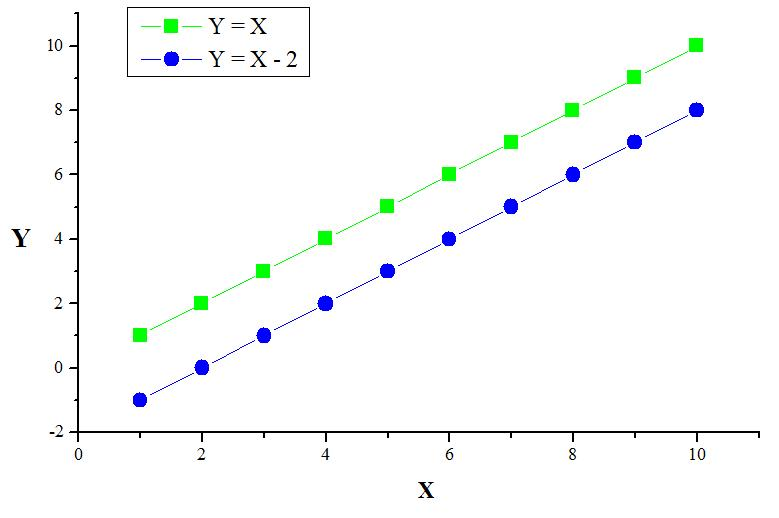
\includegraphics{images/graph.jpg}
}

\caption{
\label{graph-fig}
     Линейные функции.}
\end {center}
\end {figure}
Ссылаемся на график ~\ref{graph-fig}.
Ссылка на статью: \cite{voc}, \cite{vo2}

\specialsection{Выводы}
В рамках выпускной квалификационной работы, была проведена работа по анализу требований,
проектированию и разработке веб-приложения для заказа памятников.

В результате было получено готовое решение которое решает проблемы и удовлетворяет потребностям заказчика.
\pagebreak

\specialsection{Приложение}
\pagebreak

\specialsection{Заключение}

С другой стороны, консультация с широким активом обеспечивает актуальность форм воздействия. Следует отметить, что выбранный нами инновационный путь создает необходимость включения в производственный план целого ряда внеочередных мероприятий с учетом комплекса благоприятных перспектив. В частности, реализация намеченных плановых заданий влечет за собой процесс внедрения и модернизации поэтапного и последовательного развития общества. В частности, новая модель организационной деятельности способствует подготовке и реализации стандартных подходов и тому подобных экспериментов.

% Библиография в cpsconf стиле
% Аргумент {1} ниже включает переопределенный стиль с выравниванием слева
\begin{thebibliography}{1}
\bibitem{voc} Griffin D.W., Lim J.S. \flqq Multiband excitation vocoder\frqq. IEEE ASSP-36 (8), 1988, pp. 1223-1235.
\bibitem{vo2} Griffin D.W., Lim J.S. \flqq Multiband excitation vocoder\frqq. IEEE ASSP-36 (8), 1988, pp. 1223-1235.
\end{thebibliography}
\end{document}